
\documentclass[10pt,a4paper]{article}

%%%%%%%%%%%%%%%%%%%%%%%%%%%%%%%%%%%%%%%%%%%%%%%%%%%%%%%%
%
% Packages and Theorem Environments

\usepackage{graphicx}
\usepackage{psfrag}
\usepackage{epsf}
\usepackage{amsmath,amsfonts,amssymb,latexsym}
\usepackage{enumitem}
\usepackage{algorithmic}
\usepackage{algorithm}
\usepackage[width=160mm,height=240mm,left=35mm,foot=10mm]{geometry}
\usepackage{xcolor}
\usepackage{url}
\usepackage{hyperref}
\usepackage{tikz}



\renewcommand{\theequation}{\thesection.\arabic{equation}}
\newcommand{\makeTiny}[1]{{\tiny #1}}
\newcommand{\work}{\tiny}
\newcommand{\ignore}[1]{}
\newcommand{\startClaims}{\setcounter{claim}{0}}
\newtheorem{theorem}{Theorem}[section]
\newtheorem{corollary}[theorem]{Corollary}
\newtheorem{lemma}[theorem]{Lemma}
\newtheorem{proposition}[theorem]{Proposition}
\newtheorem{conjecture}[theorem]{Conjecture}
\newtheorem{problem}[theorem]{Problem}
\newtheorem{question}[theorem]{Question}
\newtheorem{definition}[theorem]{Definition}
\newtheorem{task}[theorem]{Task}
\newtheorem{claim}{Claim}
\newtheorem{remark}[theorem]{Remark}
\newtheorem{observation}[theorem]{Observation}

\DeclareUnicodeCharacter{2212}{-}
\graphicspath{hw4}



\title{MATH 351--004 -- Assignment \#$4$\\
}

\author{Alex Iacob\\
ai9388}

\date{September 23, 2021}


%%%%%%%%%%%%%%%%%%%%%%%%%%%%%%%%%%%%%%%%%%%%%%%%%%%%%%%%
%
% Author's definitions


\newcommand{\NN}{\mathbb N}
\newcommand{\ZZ}{\mathbb Z}
\newcommand{\QQ}{\mathbb Q}
\newcommand{\RR}{\mathbb R}

\newcommand{\BB}{\mathcal B}
\newcommand{\ZT}{\mathcal Z}

\newcommand{\Cl}{\operatorname{Cl}}
\newcommand{\Bd}{\operatorname{Bd}}
\newcommand{\row}{\operatorname{row}}
\newcommand{\col}{\operatorname{col}}
\newcommand{\Span}{\operatorname{span}}
\newcommand{\convhull}{\operatorname{conv.hull}}
\newcommand{\tr}{\operatorname{tr}}

\newcommand{\diam}{\operatorname{diam}}

\begin{document}

\maketitle

\subsection*{Problem 1 - Prove that every connected graph all of whose vertices have even degrees contains no bridges}
If we were to consider Graph G with all even degree vertices.
Somewhere in this graph, there is this bridge that joins vertex $x$ to vertex $y$. Upon removing this edge, there are two subgraphs of $G$, $G_{x}$ and $G_{y}$. If we were to consider $G_{x}$, then $G_{x}$ has exactly one vertex with an odd degree and the rest have even degrees. This creates a contradiction of Corollary 2.3, thus every connected graph all of whose vertices have even degrees contains no bridges.


\subsection*{Problem 2 - Let $G$ be a connected graph that $e_{1}$ and $e_{2}$ be two edges of $G$. Prove that 
$G - e_{1} - e_{2}$ has three components if and only if both $e_{1}$ and $e_{2}$ are bridges in $G$.}

Forward:\\
By definition, G is connected, therefore it has one connected component. \\
Since $e_{1}$ is a bridge, by definition, $G - e_{1}$ would contain two connected components.\\
However, we do not know if $e_{2}$ is a bridge in $G - e_{1}$. Using Theorem 4.1, we know that if $e$ is a bridge in $G$ and $e \in H \subseteq G$, then $e$ is a bridge of $H$. Therefore we know that $e_{2}$ is a bridge in $G - e_{1}$, which would make the total connected components equal to 3.\\
Backward:\\
If $G - e_{1} - e_{2}$ has 3 connected components, then edges $e-{1}$ and $e_{2}$ are bridges. \\
Using the formula $\kappa(G) \leq \kappa(G - e) \leq \kappa(G) + 1$.
Suppose that e1 is not a bridge, then we know that\\
$\kappa(G - e_{1}) = 1$\\
$1 \leq \kappa((G - e_{1}) - e_{2}) \leq 2$\\ Contradiction
Suppose that e2 is not a bridge, then we know that\\
$\kappa(G - e_{1}) = 2$\\
$2 \leq \kappa((G - e_{1}) - e_{2}) \leq 3$\\ 
$\kappa((G - e_{1}) - e_{2}) = 3$


\subsection*{\newpage Problem 3 - A certain tree $T$ of order 35 is known to have 25 vertices of degree 1, two vertices of degree 2, three vertices of degree 4, one vertex of degree 5 and two vertices of degree 6. It also contains two vertices of the same (unknown) degree $x$. What is $x$? }

Via the Handshake Lemma and knowing that size of tree is its order - 1 (and also featuring my artistic talent)\\
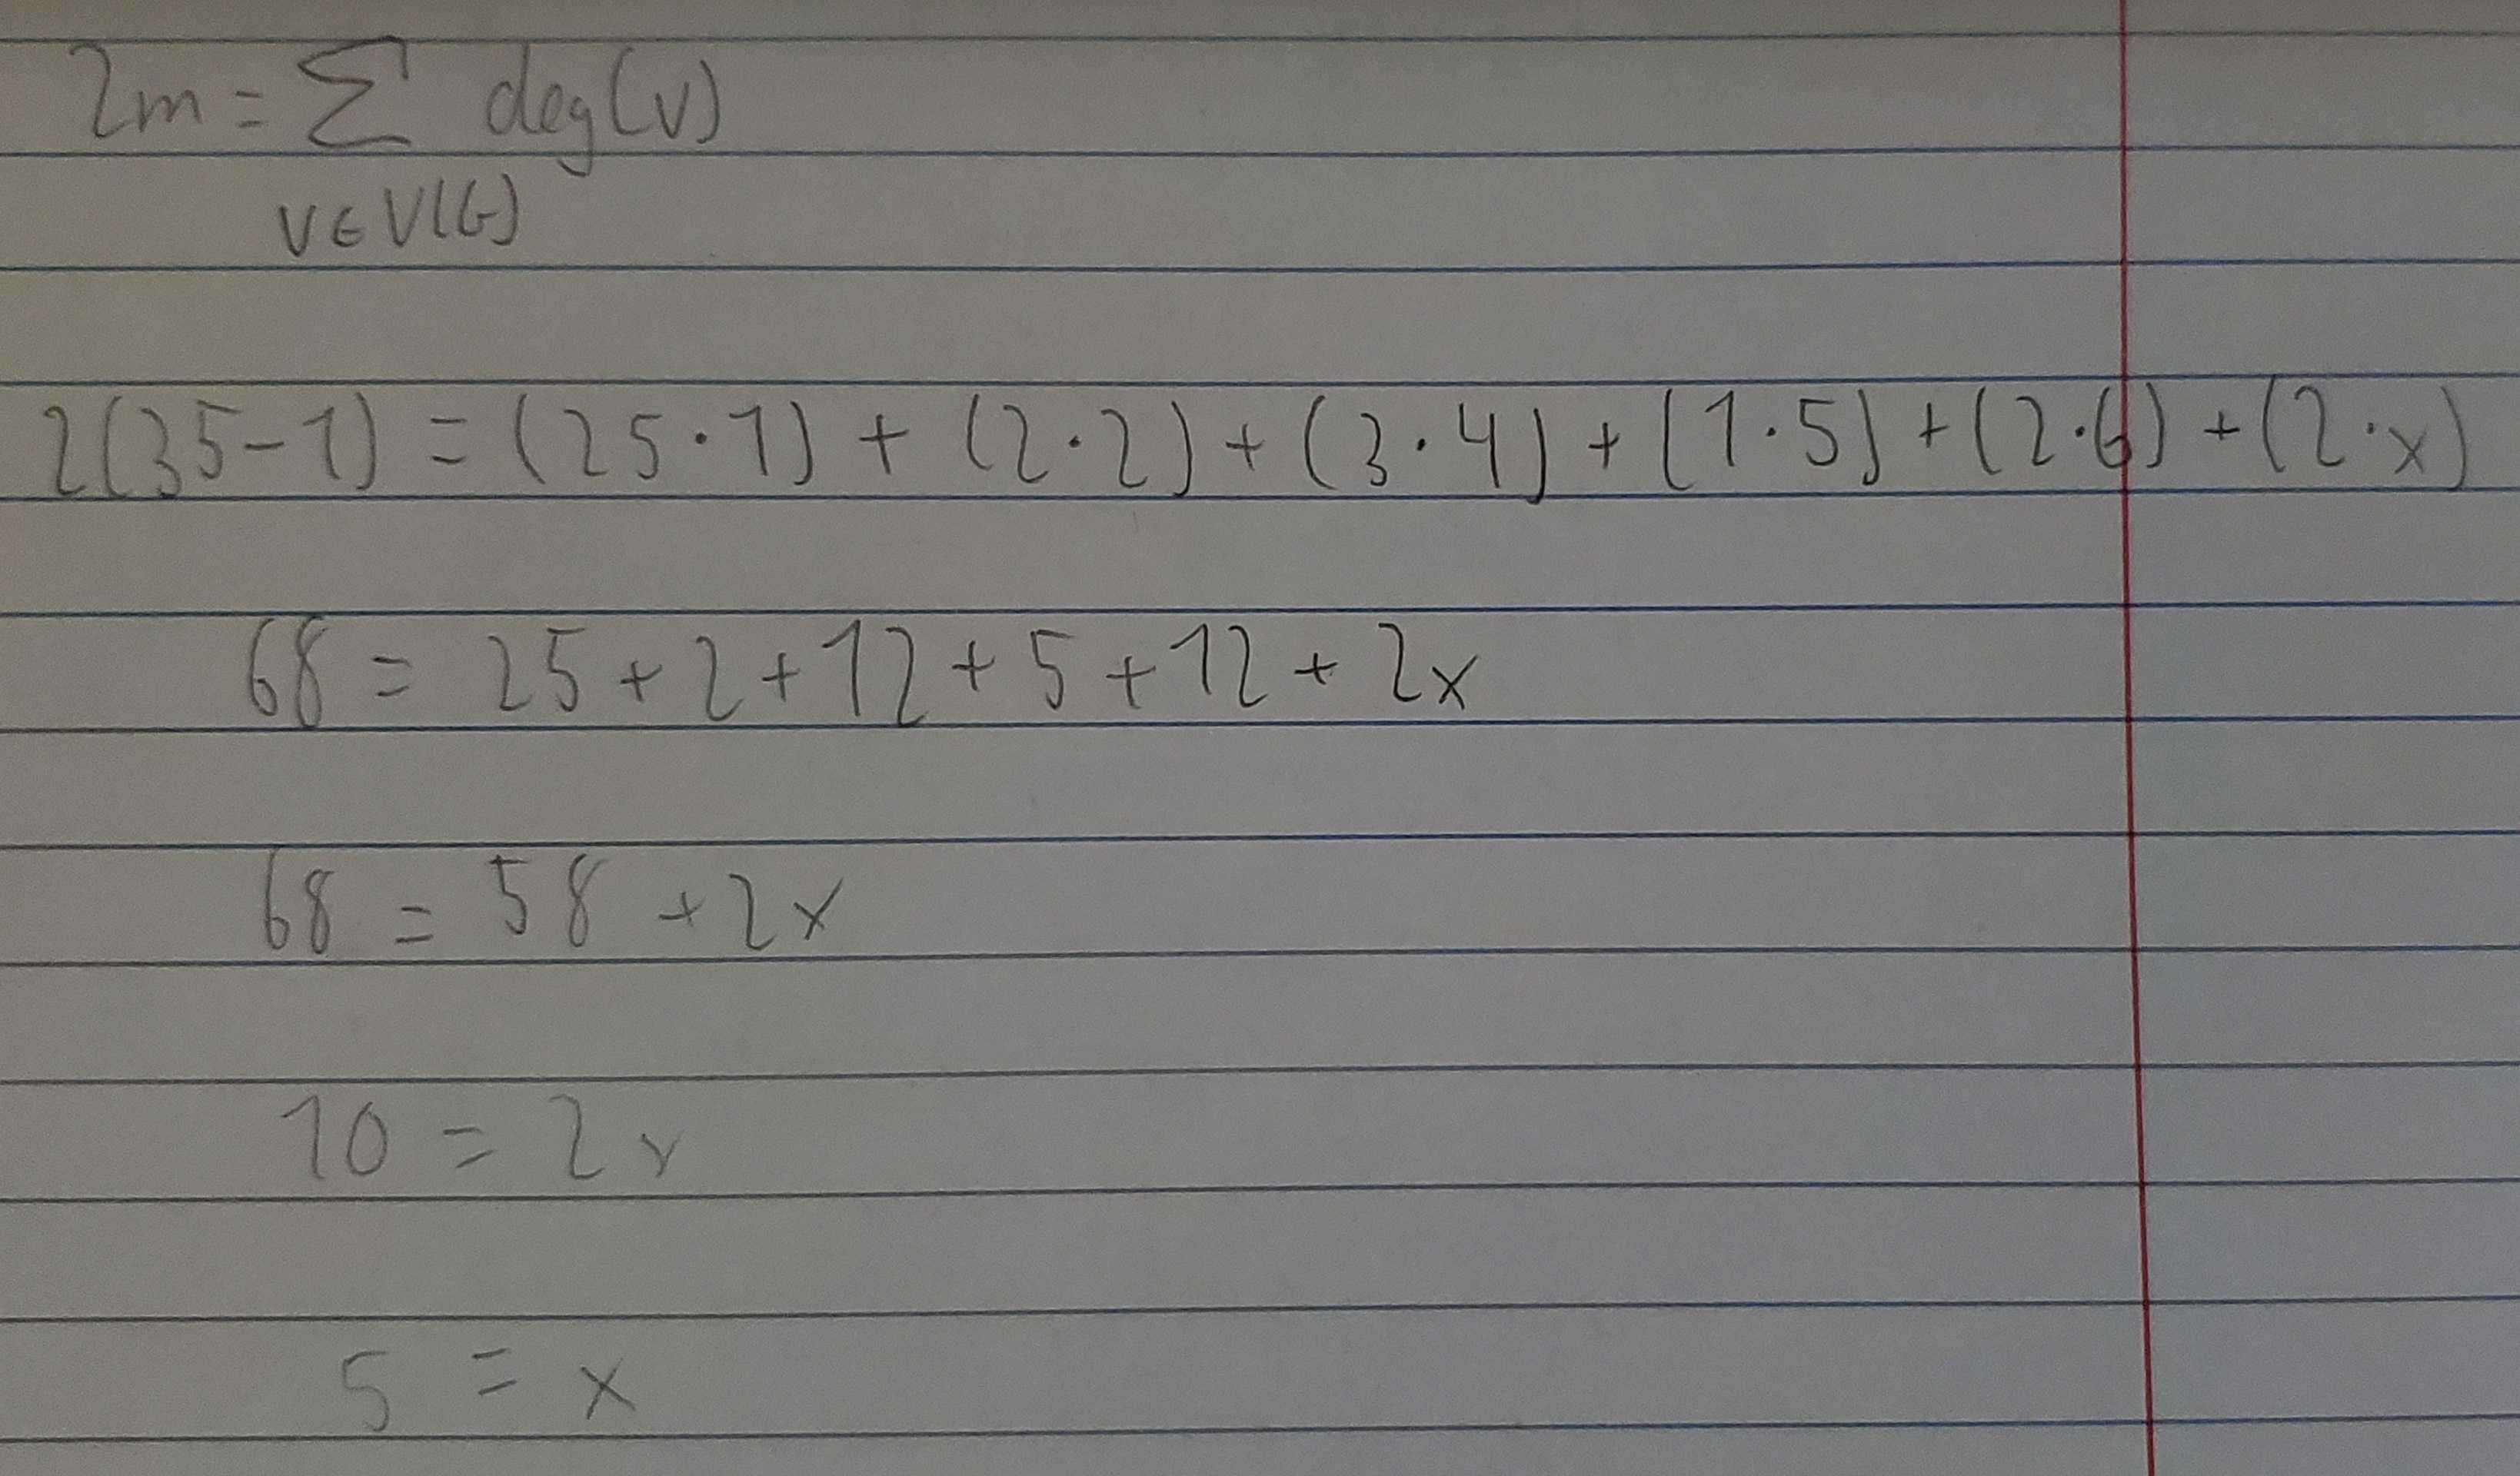
\includegraphics[width = 10cm]{question3_calculation}\\
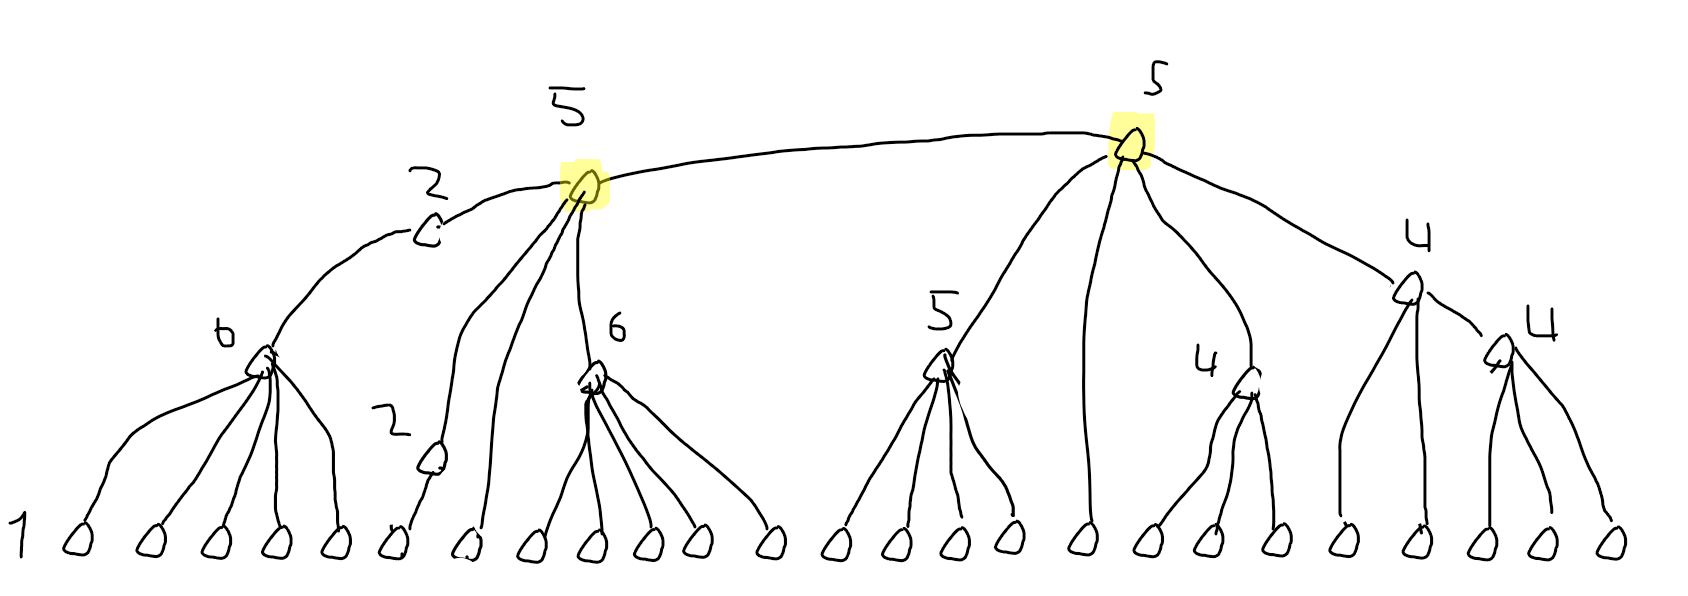
\includegraphics[width = 10cm]{question3_image}\\

\subsection*{Problem 4 - A certain tree $T$ of order $n$ contains only vertices of degree 1 and 3. Show that T contains $(n − 2)/2$ vertices of degree 3}

Let $x$ = the amount of vertices with degree 1.\\
Let $y$ = the amount of vertices with degree 3.\\
$x + y = n$\\
$x + 3y = 2n - 2$

\end{document} 




















